% example.tex
\documentclass[dvisvgm]{standalone}

\usepackage{amsmath}
\usepackage[usenames,dvipsnames]{xcolor}
\usepackage{tikz}
\usetikzlibrary {arrows.meta,
                 positioning,
                 shapes.geometric}

 \tikzset{
        base/.style={draw, align=center, minimum height=4ex},
        proc/.style={base, rectangle, text width=8em},
        io/.style={trapezium, trapezium left angle=70, trapezium right
                   angle=110, draw, text width=8em, %minimum width=2cm, 
                   %minimum height=1cm
                   },
        test/.style={base, diamond, aspect=2,
                     %text width=5em
                     },
        term/.style={proc, rounded corners},
        myarrow/.style={-Stealth, line width=0.25mm},
 }

\begin{document}
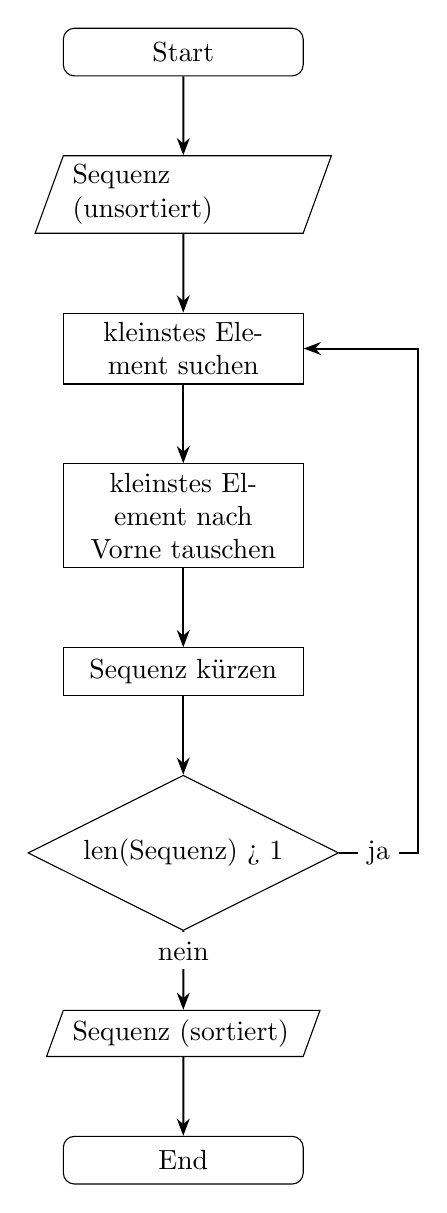
\begin{tikzpicture}
    \node[draw, term] (a) {Start};
    \node[draw, io, below= of a] (b) {Sequenz \\ (unsortiert)};
    \node[draw, proc, below= of b] (c) {kleinstes Element suchen};
    \node[draw, proc, below= of c] (d) {kleinstes Element nach Vorne tauschen };
    \node[draw, proc, below= of d] (e) {Sequenz kürzen};
    \node[draw, test, below= of e] (f) {len(Sequenz) > 1};
    \node[draw, io, below= of f] (g) {Sequenz (sortiert)};
    \node[draw, term, below= of g] (h) {End};

    \draw[myarrow] (a) edge (b);
    \draw[myarrow] (b) edge (c);
    \draw[myarrow] (c) edge (d);
    \draw[myarrow] (d) edge (e);
    \draw[myarrow] (e) edge (f);
    \draw[myarrow] (f) edge node [near start, fill=white] {nein} (g);
    \draw[myarrow] (g) edge (h);

    \draw[myarrow] (f.east) -| node [near start, fill=white] 
                   {ja} ++(1,0) |- (c.east);
\end{tikzpicture}
\end{document}
